\documentclass[14pt]{amsart}
%\usepackage{amsmath}
\usepackage[utf8]{inputenc}
\usepackage{graphicx}
\usepackage{xcolor}
\usepackage[legalpaper, margin=1.0in]{geometry}
\usepackage{fancyvrb}
\usepackage{cprotect}
\usepackage{url}
\usepackage{etoolbox}
\usepackage{hyperref}
\usepackage[skins,theorems]{tcolorbox}
\usepackage{enumitem}
\newcommand*{\vertbar}{\rule[-1ex]{0.5pt}{2.5ex}}
\newcommand*{\horzbar}{\rule[.5ex]{2.5ex}{0.5pt}}
\setlist[itemize]{align=parleft,left=1pt..1em}

\usepackage{imakeidx}
\makeindex


\usepackage{cmbright}
\usepackage[OT1]{fontenc}


% fonts
%\input{ArtNouvc.fd}
%\newcommand*\initfamily{\usefont{U}{ArtNouvc}{xl}{n}}
%\usepackage[T1]{fontenc}
%\usepackage{tgbonum} % change font

%\usepackage[light,condensed,math]{iwona}
%\usepackage[T1]{fontenc}

% from https://www.pinterest.co.uk/pin/88664686405122253/
\definecolor{C1}{RGB}{141, 125, 158} %purple
\definecolor{C2}{RGB}{163,156,147} % yellow
\definecolor{C3}{RGB}{99,151,153} % green
\definecolor{C4}{RGB}{195,106,99} % red
\definecolor{C5}{RGB}{124, 132, 128}
\definecolor{C6}{RGB}{67, 69, 75}


\definecolor{Gr}{HTML}{377D71}
\definecolor{Pu}{HTML}{A459D1}
\definecolor{Bl}{HTML}{4D455D}
\definecolor{Te}{HTML}{C1ECE4}
\definecolor{Or}{HTML}{EF6262}
\definecolor{Am}{HTML}{F3AA60}
\definecolor{Co}{HTML}{3C486B}
\definecolor{Wh}{HTML}{FEFBF6}
\definecolor{Ye}{HTML}{FFE196}
\definecolor{Re}{HTML}{E96479}
\definecolor{Pi}{HTML}{FFD0D0}
\definecolor{Rp}{HTML}{FF9EAA}
\definecolor{Wg}{HTML}{EEF3D2}


\hypersetup{
    colorlinks=false,
    linkcolor=red,
    filecolor=red,      
    urlcolor=red,
    pdftitle={a},
    pdfpagemode=FullScreen,
    }
    
    
 % TCOLORBOX STUFF ----------------------------------------------------------------------------
 

 %  ----------------------------------------------------------------------------
    
\patchcmd{\section}{\normalfont}{\color{C5}}{}{}
\patchcmd{\subsection}{\normalfont}{\color{C5}}{}{}


\newcommand{\dfn}[1]{{\bf  \color{blue}{#1}}}


\renewcommand{\FancyVerbFormatLine}[1]{\color{gray}{>\,\,#1}}
    
\newtheorem{thm}{Theorem}


\newtheoremstyle{exercise}
{}                % Space above
{}                % Space below
{\color{black}}        % Theorem body font % (default is "\upshape")
{}                % Indent amount
{\bfseries}       % Theorem head font % (default is \mdseries)
{:}               % Punctuation after theorem head % default: no punctuation
{ }               % Space after theorem head
{}                % Theorem head spec
\theoremstyle{exercise}
\newtheorem{exercise}{Exercise}


\newtheoremstyle{example}
{}                % Space above
{}                % Space below
{\color{red}\slshape}        % Theorem body font % (default is "\upshape")
{}                % Indent amount
{\bfseries}       % Theorem head font % (default is \mdseries)
{.}               % Punctuation after theorem head % default: no punctuation
{ }               % Space after theorem head
{}                % Theorem head spec
\theoremstyle{example}
\newtheorem{example}{Example}

\newtheoremstyle{solution}
{}                % Space above
{}                % Space below
{\color{C5}}        % Theorem body font % (default is "\upshape")
{}                % Indent amount
{\bfseries }       % Theorem head font % (default is \mdseries)
{:}               % Punctuation after theorem head % default: no punctuation
{\newline}               % Space after theorem head
{}                % Theorem head spec
\theoremstyle{solution}
\newtheorem*{solution}{Solution}


\newcommand{\mcS}{\mathcal S}
\newcommand{\mcR}{\mathcal R}
\newcommand{\mcC}{\mathcal C}
\newcommand{\bS}{{\boldsymbol S}}
\newcommand{\bR}{{\boldsymbol R}}
\newcommand{\bC}{{\boldsymbol C}}
\newcommand{\ba}{{\boldsymbol a}}
\newcommand{\bb}{{\boldsymbol b}}
\newcommand{\bs}{{\boldsymbol s}}
\newcommand{\bff}{{\boldsymbol f}}
\newcommand{\br}{{\boldsymbol r}}
\newcommand{\bx}{{\boldsymbol x}}
\newcommand{\bt}{{\boldsymbol t}}
\newcommand{\bv}{{\boldsymbol v}}
\newcommand{\bu}{{\boldsymbol u}}
\newcommand{\bw}{{\boldsymbol w}}
\newcommand{\bc}{{\boldsymbol c}}
\newcommand{\be}{{\boldsymbol e}}
\newcommand{\bq}{{\boldsymbol q}}
\newcommand{\bphi}{{\boldsymbol \phi}}
\newcommand{\brho}{{\boldsymbol \rho}}
\newcommand{\btau}{{\boldsymbol \tau}}
\newcommand{\reals}{\mathbb R}
\newcommand{\ints}{\mathbb N}
\newcommand{\E}{\mathbb E}
\newcommand{\Prob}{\mathbb P}


%%%%%%%%%%%%%%%




\begin{document}

\title{Expectation and variance, Binomial distribution, continuous distributions}

\maketitle
\tableofcontents

\section{Reading}
\begin{itemize}
%\item Read section 2.4 from \cite{islp}.
\item Read sections 2.8 and 3.1 \cite{tabak}
\end{itemize}

\section{Learning objectives}

\begin{itemize}
\item Familiarity with expectations and variances 
\item Familiarity with the binomial distribution and using it as a model for data. 
\item The Law of large numbers and ``soft''  Central limit theorem
\item Understanding of continuous probability distributions and what a probability density is.
\item Normal distribution
\end{itemize}




\section{Expectation and  variance}




\subsection{Sample averages and expectation}
\begin{itemize}
\item Usually it is difficult to obtain the full distribution of a random variable from data and it may not even be that relevant for the questions we are asking. Instead, we would like to summarize properties of a random variable from \dfn{statistics}. The simplest example is the \dfn{sample mean} or \dfn{sample average}. 
If we have many samples $Y_1,Y_2,\dots,Y_n$ of a random variable $Y$ (e.g. answers to a survey question), the sample mean is defined as
\begin{equation*}
\overline{Y} = \frac{1}{n}\sum_{i=1}^nY_i
\end{equation*}
More generally, we might look at the average of some function of a random variable 
\begin{equation*}
\overline{f(Y)} = \frac{1}{n}\sum_{i=1}^nf(Y_i)
\end{equation*}
\item  These sample means can be computed from the probability distribution.  Suppose each $Y_i$ can take on outcomes $Y = 1,2,3,\dots,m$. If $n$ is large, then the fraction of samples for which $Y_1= y$ will be $P(Y_1=y)$, thus the sample mean converges to the true mean: 
 \begin{equation*}
\overline{Y} =  \frac{1}{n}\sum_{i}Y_i = \frac{1}{n} \sum_{y=1}^m y n_i=\sum_{y=1}^m y \frac{n_i }{n}\approx  \sum_{y=1}^m y P(Y=y)
\end{equation*}
\item Sometimes we write $P(Y_i = y_i)$ and sometimes we write 
The expression on the right is the definition of the mean, or \dfn{expectation} denoted $E[Y]$.
\item In many cases we would like to measure deviations from the mean. For this we look at the \dfn{variance},
\begin{equation*}
{\rm var}(Y) = E[(Y-E[Y])^2]
\end{equation*}
Another way to write this is 
\begin{equation*}
 {\rm var}(Y) = E[Y^2] - 2E[Y]^2 + E[Y]^2 = E[Y^2]-E[Y]^2
\end{equation*}
We can of course estimate this from a large number of samples, although as we will later see the obvious way of doing this by replacing the expectations with sample averages is not optimal. The square root of the variance is called the \dfn{standard deviation}. 

%For this, we have the  \dfn{sample variance}
%\begin{equation}
%\sigma^2 = \frac{1}{n-1}\sum_{i}(y_i-\bar{y})^2.
%\end{equation}
% For large $n$, this converges to the square root of the \dfn{variance}
%\begin{equation}
%{\rm Var}(Y) = \sum (y_i - \E[Y])^2 P(Y_i=y_i).
%\end{equation}
%\item The sample standard deviation is
%\begin{equation}
%\sigma = \sqrt{\frac{1}{n-1}\sum_{i}(y_i-\bar{y})^2}.
%\end{equation}
%\item In python, functions for implementing the mean and standard deviation are follows:
%\begin{Verbatim}
%np.mean(y)
%np.std(y)
%\end{Verbatim}
%By default, the standard deviation function divides the sum by the number of samples, we can fix this 
%\begin{Verbatim}
%np.std(y,ddof=1)
%\end{Verbatim}
\end{itemize}


\begin{example}[Mean and variance of Bernoulli random variable]
Let $Y$ be a Bernoulli random variable with parameter $q$. We will use the convention that $Y=1$ with probability $q$.\\


\noindent
\underline{Question}: What is $E[Y]$ and ${\rm var}(Y)$?\\

\noindent
\underline{Solution}: Using the definitions above
\begin{equation*}
E[Y] = P(Y=0)\times 0 + P(Y=1)\times 1 = q
\end{equation*}
similarly you should be able to see that ${\rm var}(Y) = q(1-q)$. 
In the python notebook we test the formula $E[Y]=q$. 
\end{example}

\subsection{Conditional expectation}
\begin{itemize}
\item We define the conditional expectation as the expectation of the conditional variable; that is, 
\begin{equation*}
\E[X|Y=y] = \sum_{x} xP(X|Y=y)
\end{equation*}
With samples
\begin{equation*}
\{(x_1,y_1),\dots,(x_n,y_n)\}
\end{equation*}
 we could obtain this from a sample by taking the sample mean of $X$ among just the samples where $y_i = y$; that is, let 
 \begin{equation*}
 n_1 = \text{number of samples where $y_i = y$}
 \end{equation*}
 then 
 \begin{equation*}
 \E[X|Y=y] \approx  \frac{1}{n_1}\sum_{i=1}^n1_{\{y_i = y\}}x_i
 \end{equation*}
 where $1_{\{y_i = y\}}$ is the \dfn{indicator function}
 \begin{equation*}
 1_{\{y_i = y\}} = \left\{ \begin{array}{cc}
 0 & \text{ if } y_i\ne y\\
  1 & \text{ if } y_i=y
  \end{array}\right.
 \end{equation*}
 \item As we already noted, the conditional probabilities can tell us whether two variables are independent. That is, $P(X|Y) = P(X)$ if and only if $X$ and $Y$ are independent. If $X$ and $Y$ are independent, then $E[X|Y=y]= E[X]$ for all $y$ but the converse is false: {\bf it is possible that this is true but $X$ and $Y$ are not independent!} We will say about this later.  
\end{itemize}




\begin{example}[Computing conditional from probability model ]
Consider the pair of random variables $(Y_A,Y_B)$ defined by the probability distribution we saw in week 1:
\begin{equation}\label{eq:gene}
P(Y_A,Y_B) = \left\{ \begin{array}{cc}
1/2 & \text{ if }Y_A=0 \text{ and } Y_B = 0\\
1/8 & \text{ if }Y_A=0 \text{ and } Y_B = 1\\
1/8 & \text{ if }Y_A=1 \text{ and } Y_B = 0\\
1/4 & \text{ if }Y_A=1 \text{ and } Y_B = 1\\
\end{array}
 \right.\\
\end{equation}


\noindent
\underline{Question}: Compute $E[Y_A|Y_B=1]$\\

\noindent
\underline{Solution}: We can obtain the conditional distribution of $Y_A$ as 
\begin{equation*}
P(Y_A=1|Y_B = 1) = \frac{P(Y_A=1,Y_B=1)}{P(Y_B=1)} = \frac{1/4}{3/8} = \frac{2}{3}
\end{equation*}
Note that his means $P(Y_A=0|Y_B = 1) = 1/3$ and so the conditional distribution of  $Y_A$ is 
\begin{equation*}
Y_A|(Y_B=1) \sim {\rm Bernoulli}(2/3)
\end{equation*}
which means 
\begin{equation*}
E[Y_A|Y_B=1] = \frac{2}{3}.
\end{equation*}

\end{example}

\begin{example}[Computing conditional expectation from data ]
Consider the following data containing children's test scores and some other information. Let $Y$ be the test score and $X$ be a binary variable representing whether the mother graduated high school.\\

% Supp
%\begin{align*}
%X &\sim {Bernoulli}(q)\\
%Y|(X=x) &\sim {\mr Normal}(\mu_1 X + \mu_2 (1-x),\sigma)
%\end{align*}

\noindent
\underline{Question}: Compute $E[Y|X=0]$ and $E[Y]$. Based on this, do you think it's likely that $X$ and $Y$ are independent? \\

\noindent
\underline{Solution}: See Python notebook.



\end{example}




  \subsection{Some additional properties of expectation}
  \begin{itemize}
   \label{prop:lin}\item Previously, I introduced the notation of expectation and we saw how to compute expectations in Python. Now we cover some addition properties. 
  \begin{enumerate}
  \item {\bf Linearity:} For two random variables $X$ and $Y$ with discrete samples spaces $S_X$ and $S_Y$, 
  \begin{equation*}
  E[X+Y] = E[X]+E[Y]
  \end{equation*}
  \begin{proof} We have 
  \begin{align*}
  E[X+Y] &= \sum_{y \in S_Y}\sum_{x\in S_X} (x+y)P(X=x,Y=y) \\
  &= \sum_{x \in S_X} \sum_{y \in S_Y} xP(X=x,Y=y)  +  \sum_{x \in S_X} \sum_{y \in S_Y} yP(X=x,Y=y) \\
  &= \sum_{x \in S_X} x\left( \sum_{y \in S_Y}P(X=x,Y=y)  \right)+   \sum_{y \in S_Y} y\left( \sum_{x \in S_X} P(X=x,Y=y)\right) \\
  &= E[X] + E[Y]
  \end{align*}
  \end{proof}
    \item {\bf Multiplication by a constant:} If $a$ is a constant (meaning it is not random), then 
    \begin{equation*}
      E[aX] =  a E[X]
    \end{equation*}
     \begin{proof}  Left as an exercise. 
     \end{proof}
  \item \label{prop:ind}  {\bf Factoring for independent variables:} If $X$ and $Y$ are independent, the 
  \begin{equation*}
  E[XY]=E[X]E[Y]
  \end{equation*}
    \begin{proof} Using independence, we have 
    \begin{align*}
     E[XY] &= \sum_{x \in S_X}\sum_{y \in S_Y} xy P(X=x,Y=y)  \\
     &= \sum_{x \in S_X}\sum_{y \in S_Y} xP(X=x)yP(Y=y) \\
     &= \left( \sum_{x \in S_X} xP(X=x)\right)\left( \sum_{y \in S_Y} yP(X=x)\right)= E[X]E[Y]
    \end{align*}
    \end{proof}
    \item {\bf Tower property:} Let $X$ and $Y$ be two random variables,  
   \begin{equation*}
   E[E[X|Y]] = E[X]
   \end{equation*}
   where by $E[X|Y]$ we mean the random variable constructed by taking the conditional expectation of $X$ given a random value of $Y$. Another way to define this is to introduce the deterministic function  $f(y) = E[X|Y=y]$ which outputs a number for every value $y \in Y$. Then we define the random variable $E[X|Y] = u(Y)$.  Therefore
   \begin{equation*}
   E[E[X|Y]]  = E[f(Y)] 
   \end{equation*}
   \begin{proof}
   Left as an exercise. 
   \end{proof}
  \end{enumerate}
  \end{itemize}
  
  
   \begin{example}[Calculating probabilities]
Consider the model probability model for a variable $X$ (similar to Equation \ref{eq:gene}) 
\begin{equation*}\label{eq:gene}
P(X) = \left\{ \begin{array}{cc}
1/2 & \text{ if }X=1\\
1/8 & \text{ if }X=2\\
1/8 & \text{ if }X=3\\
1/4 & \text{ if }X=4
\end{array}
 \right.\\
 \end{equation*}
 and define 
 \begin{equation*}
 Y = X\cdot Z,\quad Z = {\rm Geometric}(1/2). 
 \end{equation*}
In this example we consider the joint distribution $(Y,X)$. \\


\noindent
\underline{Question}: Using simulations of this model, illustrate properties of expectation in Python.\\

\noindent
\underline{Solution}: See Python notebook. The one that requires the most explanation is the tower property.
We will use simulations to show. Let $(X_1,Y_2),\dots,(X_N,Y_N)$ be our samples. We will show that $E[X] = E[E[X|Y]]$. The left hand side is easy to approximate with samples -- just take the mean of the $X$ values. To compute $E[X|Y]$ we need to compute $E[X|Y=y]$ for each $y$. If $n_y$ is the number of samples such that $Y_i=y$ then 
\begin{equation*}
E[X|Y=y] \approx \frac{1}{n_y}\sum_{\{i:Y_i =y\}}X_i
\end{equation*}
The sum is over all the $Y_i$ for which $Y_i=y$. We could also write this sum as $\sum_{i=1}^NX_i1_{Y_i=y}$. 
This means 
\begin{equation*}
E[E[X|Y]] \approx E\left[ \frac{1}{n_y}\sum_{\{i:Y_i =Y\}}X_i  \right] = \sum_{y \in S_y}P(Y=y)\underbrace{\left(\frac{1}{n_y}\sum_{\{i:Y_i =y\}}X_i  \right)}_{\approx E[X|Y=y]}
\end{equation*}
Now use that $P(Y=y) \approx n_y/N$, therefore 
\begin{equation*}
E[E[X|Y]]  \approx \sum_{y \in S_y}\frac{1}{n_y}\sum_{\{i:Y_i =y\}}X_i  \frac{n_y}{N}
\end{equation*}
Notice that when we cancel the $n_y$ terms we just get the usual sample mean of $X$: 
\begin{equation*}
E[E[X|Y]]  \approx \frac{1}{N} \sum_{y \in S_y}\sum_{\{i:Y_i =y\}}X_i   =  \frac{1}{N}\sum_{i=1}^NX_i = \overline{X} \approx E[X]
\end{equation*}

 \end{example}
 

  \section{Binomial Distribution}
  \begin{itemize}
  \item Suppose 
  \begin{equation*}
  Y_i \sim {\rm Bernoulli}(q),\quad i =1,\dots, N
  \end{equation*} 
  are independent. We will use the convention that $Y_i=1$ with probability $q$. Let
\begin{equation*}
Y = \sum_{i=1}^N y_i
\end{equation*}
 Then we say $Y$ follows \dfn {binomial distribution} and write
\begin{equation*}
Y \sim {\rm Binomial}(N,q)
\end{equation*}

 
 
 \begin{example}[Calculating probabilities]
Let $N=3$ and $k=2$. \\

\noindent
\underline{Question}: Calculate $P(Y=2)$?\\

\noindent
\underline{Solution}: There are 3 possible sequences that give $Y=2$. 
\begin{equation*}
(1,0,1),(1,1,0),(0,1,1)
\end{equation*}
The probability that we see any particular one of these is $(1-q)q^2$. For example, 
\begin{align*}
P(y_1 = 1,y_2 = 0,y_3 = 1) &= P(y_1 = 1)P(y_2=0)P(y_3 =1) \\
&= q(1-q)q = q^2(1-q).
\end{align*}
Therefore the chance to observe $Y=2$ with $N=3$ is
\begin{equation*}
P(Y=2) = P((1,0,1)) +P((1,1,0))  + P((0,1,1))  =  3q^2(1-q). 
\end{equation*}


 \end{example}
 
 Note that the binomial distribution has two parameters, $N$ and $q$, representing the number of flips and probability of success respectively. 
\item Now let's think about what the probability distribution will look like. The chance to find any {\bf particular} configuration of $k$ ones is 
\begin{equation*}
q^k(1-q)^{N-k}
\end{equation*}
 because they are independent. \\
 
 \noindent
However, we need to account for the fact that there are many configurations with $k$ ones. In general, there are 
\begin{equation*}
{N \choose k} = \frac{N!}{k!(N-k)!} = \frac{N \times (N-1) \times (N-2) \times \cdots \times (N-k+1)}{k \times (k-1) \times (k-2) \times \cdots \times 1}
\end{equation*}
way to have $k$ ones among $N$ samples. 
\footnote{To better understand the formula above, let $C_{N,k}$ denote the number of sequences with $k$ ones. We can break $C_{N,k}$ up into the number of terms for which $1$ appears as the first element of the sequence and those for which zero is the first. If one comes first, we have $N-1$ remaining slots to place $k-1$ ones, thus there are $C_{N-1,k-1}$ of these sequences. Similarly, if zero comes first, we have $N-1$ slots but now all $k$ ones to place, thus there are $C_{N-1,k}$ of these. It follows that 
\begin{equation*}
C_{N,k} = C_{N-1,k-1} + C_{N-1,k}. 
\end{equation*}
Notice that the quantity $C_{N,k}$ will be smallest when $k=1$ or $k=N$, since in these cases there is only one way to configure the sequence: $C_{N,1} = C_{N,N} = 1$.  You can solve the recursion to obtain the formula. }
%
%Similarly, $C_{N,N-1}= N$
%\begin{equation*}
%C_{N,N-1} = C_{N-1,N-2} + C_{N-1,N-1} \implies N = N-1 + 1
%\end{equation*}

This implies 
\begin{equation*}
P(Y=k)=  {N \choose k}q^{k}(1-q)^{N-k}. 
\end{equation*}
A graph of this function looks like a bell curve when $N$ is large -- we will see this in Python. Let's explore binomial random variables in python.  


%
% \begin{example}[Binomial distribution in python]
% Let's explore binomial random variables in python. 
% \end{example}
 
\begin{example}[Expectation of binomial]\label{ex:binomial_stats}
Let $Y$ be a binomial random variable. \\
 
 \noindent
\underline{Question:} What are $E[Y]$ and ${\rm var}(Y)$?\\
 
 
  \noindent
\underline{Solution:} 
\begin{equation*}
E[Y] = \sum_{k=1}^N k P(Y=k) =\sum_{k=1}^N k  {N \choose k}q^{k}(1-q)^{N-k} = \cdots. 
\end{equation*}
A much easier way is to use the definition of a Binomial random variable and exceptions 
\begin{align*}
E[Y] &= E\left[\sum_{j=1}^NX_i\right]\\
& \underset{(1)}{=}  \sum_{j=1}^NE\left[X_i\right]  =Nq
\end{align*}
where we are using the fact that averages are additive (property (1)). Similarly, 
\begin{align*}
E[Y^2] &= E\left[\left(\sum_{j=1}^NX_i\right)^2\right] = E\left[\sum_{i=1}^N\sum_{j=1}^NX_iX_j\right] \\
&\underset{(1)}{=}  \sum_{i=1}^N\sum_{j=1}^NE[X_iX_j]\underset{(3)}{=} \sum_{i=1}^N\sum_{j \ne i}^Nq^2 +  Nq(1-q) + Nq^2\\
&= N(N-1)q^2 + Nq(1-q)  +  Nq^2 = Nq(1-q)  + N^2q^2
\end{align*}
Therefore 
\begin{equation*}
{\rm var}(Y) =E[Y^2]-E[Y]^2 =  Nq(1-q)
\end{equation*}
\end{example}
 
To summarize what we learned in Example \ref{ex:binomial_stats}
\begin{equation}\label{eq:binomial_meanvar}
E[Y] = qN \quad\quad{\rm var}(Y) = Nq(1-q). 
\end{equation}


 

\item The important observation that the mean grows much faster with $N$ than the variance is also captured by the coefficient of variation: 
\begin{equation*}
{\rm CV} = \frac{\sqrt{{\rm var}(Y)}}{\E[Y]} = \sqrt{\frac{(1-q)}{q} \frac{1}{N}}. 
\end{equation*}
The idea is that we are measuring the variation \emph{relative} to the average. This is relevant for many applications where we only care about the relative deviations. 

%\item 
% Binomial samples can be generated in numpy with
% \begin{Verbatim}
%y = np.random.binomial(n,p,n_samples)
% \end{Verbatim}
 %\item Often we are interested not in $Y$, but the fraction $\phi = Y/N$. For example, we might be interested in the vote share in an election. 
 
 \begin{example}[Election modeling]
 Consider a model of votes in an election involving two candidate. Let $q$ be the fraction of people in the population who support candidate one and suppose $N$ people vote at the election (you can assume $N$ is much less than the total number of people in the population, as voter turnout is low). Then the number of people, $M$, who vote for the first candidate can be modeled as 
\begin{equation*}
M \sim {\rm Binomial}(N,q)
\end{equation*}
Think about the assumption we are making when we use this model. \\

 \noindent
\underline{Question:} Suppose there is a city in which a fraction $q = 0.51$ of people support a candidate for city council. If $N=1000$ people turnout for the election, what is the chance that the actual vote share, $\phi = M/N$, differs from the actual fraction of support throughout the population by more than $1\%$?\\

 \noindent
\underline{Solution:} See the Python notebook.
\end{example}

\item In the problem above the vote share is the same as the sample mean:
\begin{equation*}
\overline{X_i} = \frac{M}{N} =  \frac{1}{N}\sum_{i=1}^NX_i
\end{equation*}
You should be able to see that $E[\phi] = q$. What about the variance? 
 \begin{equation*}
{\rm var}(\phi) = {\rm var}(Y/N) = \frac{1}{N^2}{\rm var}(Y) = \frac{q(1-q)}{N}
 \end{equation*}
 Notice that this will tend towards zero as $N \to \infty$. Meanwhile, $E[\phi]$ has no dependence on $N$. This is a consequence of the fact that the CV is decreasing with $N$ and it allows us to determine $q$ by approximating $E[\phi]$ with the sample mean.
 % \begin{example}
%%\href{https://colab.research.google.com/drive/1PPFwE4GUzsr707s3mPhGRs7-TYlHxND2#scrollTo=oaFLfi0JI4in&line=1&uniqifier=1}{Coefficient of variation}
%\end{example}
%
% \begin{exercise}
%\href{https://colab.research.google.com/drive/1PPFwE4GUzsr707s3mPhGRs7-TYlHxND2#scrollTo=vAmv5zV7gfE0}{Generating binomial samples}
%\end{exercise}
%\item You should recognize that the assumption of independence is very important here. In the exercises you will see an instance where this may break down for an election model. It is a bit contrived, but contrived examples, which we sometimes refer to as \dfn{toy models}, can be very helpful when it comes to building our intuition. 
\end{itemize}





% \begin{example}[Election model in a subdivided population]
% 
% Suppose a state is divided into $L$ districts labels $i=1,\dots,L$. The $i$th district has 
% \end{example}


 \section{Law of large numbers and ``soft'' CLT}
 
 \begin{itemize}
 \item The binomial distribution illustrates a very basically principle that we have already used a number of times: When we sum over a large number of independent random variables and divide by the total number, the result is close to the mean. This is the Law of Large Numbers (LLN). 
 \begin{thm}[Law of Large numbers] Let $X_i$ be independent and identically distributed and set
 \begin{equation*}
 S_N = \sum_{i=1}^N X_i.
 \end{equation*}
 If $E[X_i]<\infty$, then $S_N/N \to E[X_i]$. 
 \end{thm}
 This is not very precise, since we should really be specific about what it means for a random number to converge to something, but for our purposes it will suffice to think of this as saying that for large enough $N$, $S_N/N$ will not differ from $E[X_i]$ very much. Another way to say this is that for iid random variables $X_i$, $i=1,\dots,N$, the sample average $\overline{X}$ approach $E[X_i]$. 
 \item The binomial distribution actually tell us more, it tell us that the variation around $E[X_i]$ is proportional to $1/\sqrt{N}$. It is natural to ask whether this is also true for other random variables. The key is that the dependence on $N$ in Equations \ref{eq:binomial_meanvar} does not depend on the distribution of $X_i$! So if $X_i$ is the roll of a dice, or a geometric distribution, we expect the same thing to hold. 
%  \begin{thm}[prerequisite to CLT] Let $X_i$ be independent and identically distributed with $E[X_i] = \mu_x<\infty$ and ${\rm var}(X_i) = \sigma_x^2<\infty$ $\sqrt{{\rm var}(S_N/N) }= \sigma_x/\sqrt{N}$. 
% \end{thm}
\item  The behavior of random sums is in-fact even more universal than this argument suggests. We can actually describe the distribution of any\footnote{With the caveat that here we only deal with the case where ${\rm var}(X_i)<\infty$} random sum with a single distribution.  In order to describe this distribution, we need to introduce the notion of continuous random variables. 
 %What we mean by ``on the order of'' is that for large enough $N$ 
 \end{itemize}

 
 
 \section{Continuous random variables}
 \begin{itemize}
 \item Here we will talk about random variables which take on continuous values. We will find that is it often easier to work with such distribution and for certain variables they are more natural models. But most importantly, the Normal model which is the foundation of so much statistical theory is a continuous variable. It emerges as an approximation of both continuous and discrete models. 
 \item  A uniform random variable, denoted  
 \begin{equation*}
 Y \sim {\rm Uniform}(a,b)
 \end{equation*}
 has an equal chance of taking any number in the interval $[a,b]$ (we assume $a<b$). Let $L=b-a$. This is distinct from other distributions we have encountered in that it is a \dfn{continuous distribution}, rather than discrete, so we need to think slightly differently about how to define the probability distribution.
 \item For the uniform distribution, 
 \begin{equation*}
 P(y_1\le Y \le y_2) = \frac{y_2-y_1}{L}
 \end{equation*}
 for $a<y_1<y_2<b$. 
 That is, the chance for $Y$ to fall in any interval is simply the length of that interval. This insures that that the probability of $Y$ being somewhere in $[a,b]$ is one: $P(a\le Y\le b) = 1$. Note that as $y_2 \to y_1$, $P(y_1\le Y \le y_2) \to 0$. This tells us that the chance for $Y$ to take any specific value is $0$. Indeed, there are simply two many number (uncountably many) in any interval to assign positive probability to each.
 
 \item  For continuous variables, it is sometimes useful to work with the density, $f(y)$ (we will use lower case letters for density and uppercase for probability distributions).The density $f(y)$ of a continuous random variable is a positive function such that 
\begin{equation*}
P(a<X<b) = \text{area under $f(y)$ between $a$ and $b$}
\end{equation*}

\item We can think of $f(y)$ as the the probability per unit $Y$, meaning that if we look in a small interval 
 \begin{equation*}
f(y)dy = P(y \le Y \le y+dy) = \frac{dy}{L}.
 \end{equation*}
 Thus, for uniform distribution the density is $1/L$ if $y \in [a,b]$ and $0$ otherwise.  Note the following properties of $f(y)$
 \begin{enumerate}
 \item It is positive
 \item The area under $f(y)$ is one (this is the continuous version of the condition that discrete probability distributions must sum to one). 
 \end{enumerate}


\begin{figure}[h]
\centering
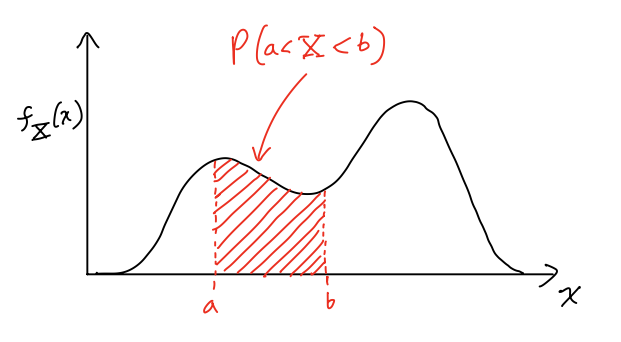
\includegraphics[width=0.6\textwidth]{./../figures/density}
\caption{The density and its relationship to probabilities}\label{fig:density}
\end{figure}



\begin{example}[Condition with continuous random variables]
If $Y$ is uniform on $[0,1]$. \\


\noindent
\underline{Question:}  What is the density of $Y|(Y<1/2)$? Check the answer with simulations.\\

 \noindent
\underline{Solution:} We can start with the definition of density
\begin{align*}
P(y_1<Y<y_2|Y<1/2) &= \frac{P(y_1<Y<y_2,Y<1/2)}{P(Y<1/2)}
\end{align*}
What is the think on the top? We will assume $y_1>0$ and $y_2<1/2$, then the numerator is $y_2-y_1$, since $Y<1/2$. The key here is that if $Y \in [y_1,y_2]$ $Y<1/2$ is automatically true, so the chance that BOTH of these things are true in a sample is the chance that the more restrictive one is true.

The denominator is $P(Y<1/2) = 1/2$. This means
\begin{equation*}
P(y_1<Y<y_2|Y<1/2) = 2(y_2-y_1)
\end{equation*}
This means the density is
\begin{equation*}
f(y|Y<1/2) = 2
\end{equation*}
Thus
\begin{equation*}
Y|(Y<1/2) \sim {\rm Uniform}(0,1/2)
\end{equation*}
We also check this with simulations in the Python notebook. 
\end{example}

%
%\begin{example}[Model with continuous and discrete variables ]
%Consider the probability model 
%\begin{align*}
%q &\sim {\rm Uniform}(0,1)\\
%X|q &\sim {\rm Binomial}(N,q)
%\end{align*}
%One way to think about this is that we are modeling the response to a survey, but we don't know what the 
%
%
%\end{example}

\item Suppose we want to model that time before a component of a machine fails. We will assume that the rate of failure -- that is, the chance that it fails per unit time -- is a constant $\lambda$. In other words, for a small time interval $dt$, the probability for the component to fail in a small time interval $[t,t+dt)$ given that it has not yet failed is $\lambda dt$. Or, in mathematical notation 
 If $T$ is the time of failure, then the density of $f_T(t)$ is 
\begin{equation*}
f_T(t) = \lambda e^{-\lambda t}.
\end{equation*}
$T$ is an \dfn{exponentially distributed} random variable, and we write
\begin{equation*}
T \sim {\rm Exponential}(\lambda).
\end{equation*}
An exponential variable has mean $E[T] = 1/\lambda$ and variance ${\rm var}(T) = 1/\lambda^2$. 



\begin{example}[Heterogeneous failure rate]

Suppose that the machine is defective with probability $0.1$. We can introduce a variable $X$ which indicates whether the machine is defective and will fail with a rate $10$. In other words, our model is 
\begin{align*}
X &\sim {\rm Bernoulli}(0.1)\\
T|(X=x) &\sim {\rm Exponential}(x10 + (1-x))
\end{align*}


\noindent
\underline{Question:} What is $E[T]$? What about ${\rm var}(T)$? Does $T$ follow an exponential distribution?\\ 


\noindent
\underline{Solution:} Using the tower property of expectation
\begin{align*}
E[T] &= E[E[T|X]] \\
&= E[T|X=0]P(X=0) + E[T|X=1]P(X=1) \\
&= 1 \cdot (1-0.1) + \frac{0.1}{10} = 0.9+0.01 = 0.91
\end{align*}
The variance 
\begin{equation*}
{\rm var}(T) = E[T^2]-E[T]^2
\end{equation*}
and 
\begin{align*}
E[T^2] = E[E[T^2|X]]  = (1-0.1)\times E[T^2|X=0] + 0.1 \times E[T^2|X=1] 
%&= 1^2 \cdot (1-0.1) +\frac{0.1}{10^2}\\
%&= 0.9 + 0.001  = 0.901
\end{align*}
Note that, from the variance formula and the fact that $T$ is exponential,
\begin{equation*}
E[T^2|X=1]  = {\rm var}(T|X=1) + E[T|X=1]^2 = \frac{1}{10^2}  + \frac{1}{10^2} = \frac{2}{10^2}
\end{equation*}
Hence 
\begin{align*}
E[T^2] = E[E[T^2|X]]  = 0.9 \cdot 2 + 0.1 \cdot \frac{2}{10^2} = 1.802
\end{align*}


\begin{equation*}
{\rm var}(T) =  1.802 -  0.91^2 = 0.9739
\end{equation*}
If $T$ is exponential, then 
\begin{equation*}
\lambda = \frac{1}{E[T]}=\frac{1}{0.91}.
\end{equation*}
We know that ${\rm var}(T) = E[T]^2$ for an exponential distribution, but 
\begin{equation*}
 \frac{1}{\lambda^2} = 0.91^2 = 0.8281 \ne  0.9739= {\rm var}(T). 
\end{equation*}


\end{example}

\end{itemize}


 \subsection{Cumulative density function}
 \begin{itemize}
\item Sometimes it is useful to characterize a continuous distribution not by the density, but by the \dfn{cumulative distribution function (CDF)}, defined as 
\begin{equation*}
F(y) = P(Y<y).
\end{equation*}
%\item What is the CDF of the uniform distribution? 
%\item The \dfn{median} is the value $y_m$ for which $F(y_m) = 1/2$. 
%\item To better understand density and CDF, imagine a student says they will arrive at my office between noon and 3. Let $Y$ represent the time a student arrives, which we will model as a Uniform random variable. Then the density is $f(y) = 1/3$ which has units 1/hours. We can think of $f$ as the rate at which the CDF increases -- that is, it is the velocity of probability.
  \end{itemize}
  
  

 \subsection{Conditional probability and expectation with Continuous variables}
 
 \begin{itemize}
 \item The definition of expected value can be generalized to continuous variables by replacing the sums with integrals. That is, for a variable $X$ with density $f_X$, we have 
 \begin{equation*}
 E[X] = \int x f_X(x)dx 
 \end{equation*}
 \item Suppose $X$ and $Y$ are two variables on the sample spaces $S_X = S_Y = \reals$. Then we can define a joint density $f_{X,Y}(x,y)$. From this, we can compute things like 
 \begin{equation*}
P(X>x,Y>y) = \int_{x}^{\infty}\int_y^{\infty}f_{X,Y}(x,y)dxdy
 \end{equation*}
 If $X$ and $Y$ are independent, then $f_{X,Y}(x,y) = f_X(x)f_Y(y)$ and 
 \begin{align*}
P(X>x,Y>y) &= \int_{x}^{\infty}\int_y^{\infty}f_{X,Y}(x,y) dx dy\\
&=  \int_{x}^{\infty}f_X(x)dx\int_y^{\infty}f_Y(y)dy
 =P(X>x)P(Y>y)
 \end{align*}
 \end{itemize}
  
  
   \subsection{The Gaussian curve}
   \begin{itemize}
   \item One of the most important probability densities it the Gaussian:
   \begin{equation*}
   f(x) = \frac{1}{\sqrt{2\pi \sigma^2}}e^{-\frac{(x-\mu)^2}{2 \sigma^2}}
   \end{equation*}

\item Despite the simplicity of the density function, calculating probabilities for Normal random variable by computing the area under the curve (integrating) is difficult. Instead we can remember some rough estimates based on the following figure. 
%As I discuss in the previous section can think of $f$ as the probability \emph{per unit of the random variable}, e.g. probability/feet.  
\begin{figure}[h]
\centering
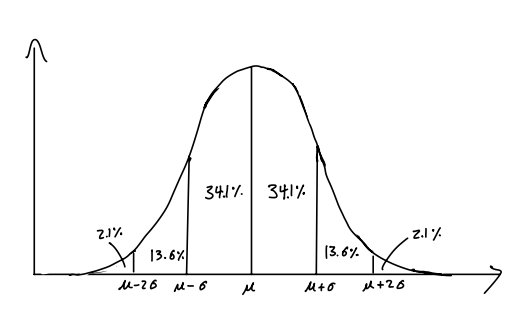
\includegraphics[width=0.6\textwidth]{./../figures/bellcurve}
\caption{Probabilities in the Normal distribution}\label{fig:bellcurve}
\end{figure}



\begin{example}[Calculating probabilities for Normal distribution]
 We use the curve above to calculate probabilities of events in the Normal distribution. Suppose
\begin{equation*}
Y \sim {\rm Normal}(5,4)\\
\end{equation*}


 \noindent
\underline{Question:} What is (approximately) $P(Y > 7)$? \\

 \noindent
\underline{Solution:} Note that $5 + 2 =  7$, so this is asking how likely it is that a Normal variable is greater than $1$ standard deviation above the mean. This about $13.5+2 = 15.5\%$. We can always easily compute these probabilities in python as well.\\ 

\noindent
%Now let
%\begin{equation*}
%Y \sim {\rm Normal}(\mu,\sigma)\\
%\end{equation*}

 \noindent
\underline{Question:} What is
\begin{equation*}
P(Y>3|Y<7)?
\end{equation*}

 \noindent
\underline{Solution:} In this case we would use
\begin{equation*}
P(Y>3|Y<7) = \frac{P(Y>3,Y<7)}{P(Y<7)} 
\end{equation*}
Notice that $3 = 5-2 = \mu-\sigma$ and we already saw $7 = 5+2 = \mu+\sigma$, so $P(Y<7) \approx 0.839$ and $P(Y>3,Y<7) \approx 0.682$, thus the result is about $0.81$. 



\end{example}

\end{itemize}





 \bibliographystyle{unsrt}
\bibliography{./../refs.bib}

  
  \end{document}
  
  